\newpage
\section{Contact Mechanics for Fully Elastic Stiff Solids}
\label{sec:solid_model}

Contact mechanics considers geometrical and surface effects to deal with material bulk properties. The effects of geometrical effects on local elastic deformations seem to have been first considered by \cite{Hertz-1882}. The developed theory of Hertzian elastic deformation links the circular contact area of a sphere with a plane or another sphere with the elastic deformation of the materials. The original framework completely disregards any surface interactions. Adhesive interactions were introduced with the \ac{JKR} theory \citep{Johnson-1971}, using a balance between the stored elastic energy and the loss in surface energy, or interface energy. 

By analyzing the stresses at the contact of two elastic solids, small strains within the elastic limit can be assumed. The contact radius $a$ is considered significantly smaller than the radius of curvature $R_i$ of the two contacting surfaces, as depicted in Figure \ref{fig:sphere_contact}

%
\begin{figure}[ht!]
	\centering 
	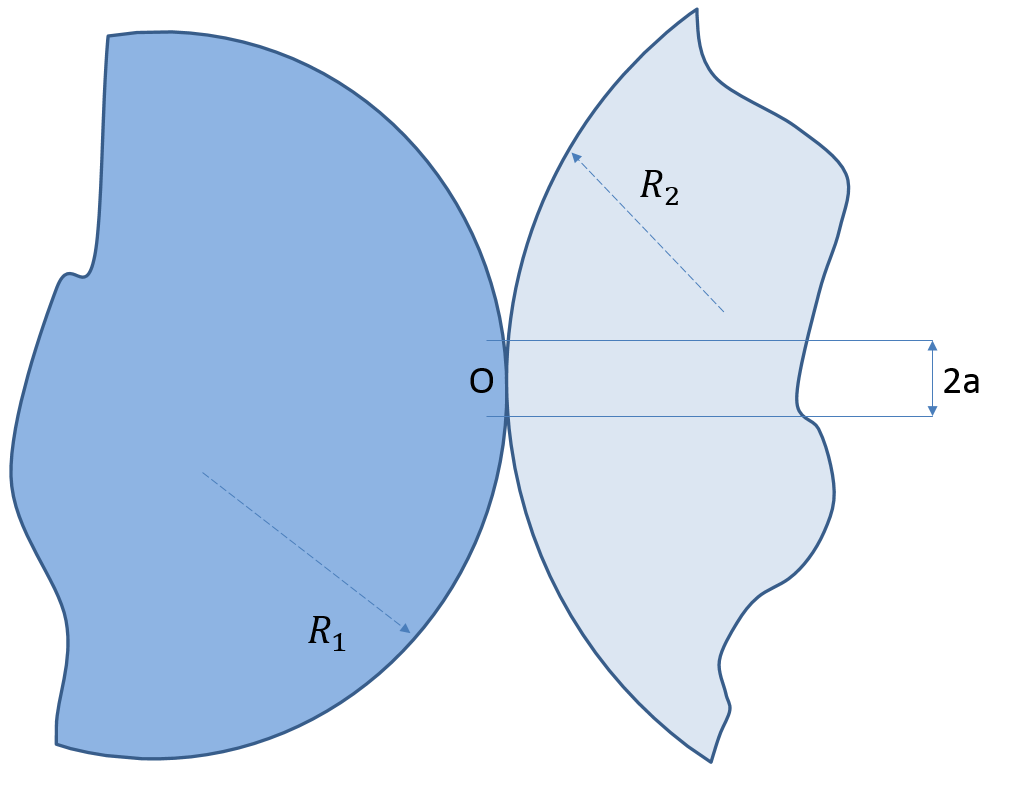
\includegraphics[width=0.55\linewidth]{Figures/2.Chapter/sphere_contact}
	\caption{Contact of two elastic spheres.}
	\label{fig:sphere_contact} 
\end{figure}
%
Assuming frictionless contact and using an elastic infinite half-space analysis, the contact radius $a$ can be written as

%
\begin{equation} \label{eq:hertz_I}
	a=\left( \frac{3FR^*}{4E^*} \right)^{\frac{1}{3}}
\end{equation}
%
where $F$ is the normal applied force, $R^*$ is the generalized radious of curvature of the interaction and $E^*$ is the generalized Young modulus, with

%
\begin{equation} \label{eq:hertz_II}
	R^*= \left( \frac{1}{R_1}+\frac{1}{R_2} \right)^{-1}; \;\;\;\; E^*= \left( \frac{1-\nu_{p1}^2}{E_1}+\frac{1-\nu_{p2}^2}{E_2} \right)^{-1}
\end{equation}
%
where $\nu_p$ is the Poisson ratio \citep{Johnson-1987}. The force is given by

%
\begin{equation} \label{eq:hertz_III}
	F=\frac{4}{3}E^*\sqrt{R^*}\delta^{3/2}
\end{equation}
%
where $\delta$ is the depth of indentation, a measure of the deformation of the sphere, given by $\delta=a^2/R^*$. The normal tension distribution (Hertz tension) can be estimated as

%
\begin{equation} \label{eq:hertz_IV}	
  p(r) = p_0\left(1-\frac{r^2}{a^2}\right)^{1/2};\;\;\;\;\;\   p_0 = \frac{3F}{2\pi a^2} = \frac{1}{\pi}\left(\frac{6F{E^*}^2}{{R^*}^2}\right)^{1/3} 
\end{equation}
%
where $r$ is the distance from the contact center.

The application of a tangential load $F_t$ to a Hertzian contact is done by assuming that normal stresses do not cause relative tangential displacements and shear stress do not produce relative normal displacements, i.e., in the absence of a tangential force, contacting points will not undergo tangential displacements \citep{Adams-2000}. It is usually assumed that, when $F_t$ is introduced, a central stick region surrounded by two slip zones is present. As the tangential force increases, the size of the stick region decreases and eventually sliding surfaces begins. This sliding respects Coulomb's friction law

%
\begin{equation} \label{eq:coulomb_friction}	
  F_t=\mu_f F_n 
\end{equation}
%
where $\mu_f$ is the friction coefficient. This law is general for static and kinetic friction, with a non-constant $\mu_f$ value. Conceptual models for the tensions developed prior to sliding are scarce. The traditional model is introduced in Chapter \ref{cap:chapter-numerical}, since it is described and assembled in discrete terms.
